\subsection{What is a Data Vault?}
\label{sec:datavault}

Data vault modelling is a database modelling methodology design that provide long-term historical storage of data coming in from multiple operational systems.
%
The base design principal is single version of the truth (SVOT) that supports data warehousing for either a single centralised database or a distributed synchronised database. This method is accomodating of change. Its adaptability provides resilience over time to changes in the data and data structures.
%
The data vault methodology is based on SEI/CMMI Level 5 best practices.
\\
\noindent
This is an example of a data vault:

\begin{figure}[H]
    \centering
    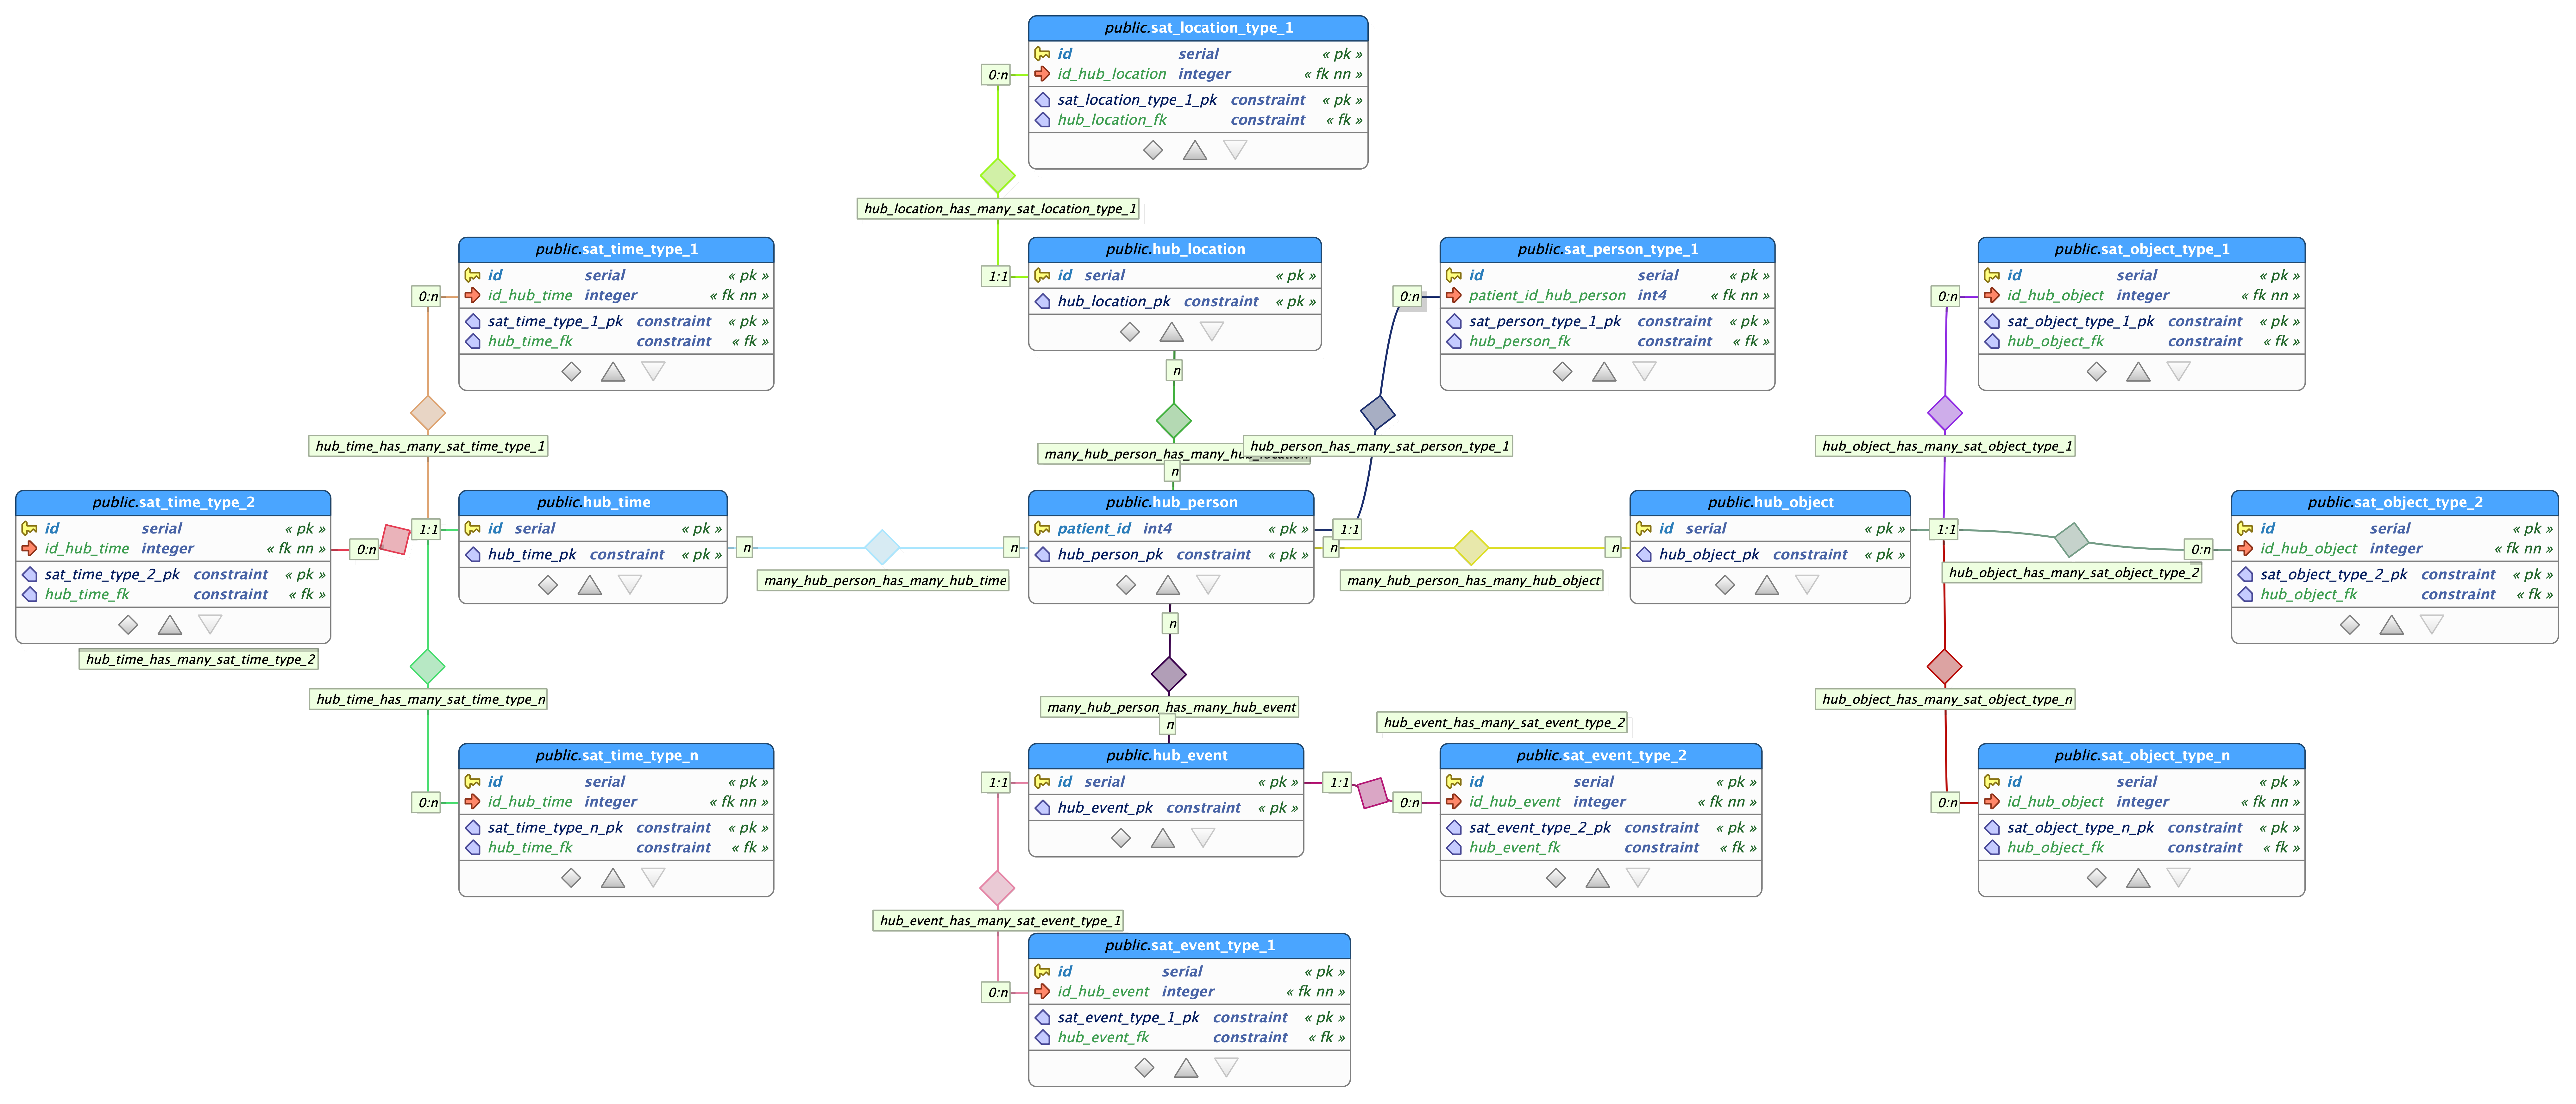
\includegraphics[width=10cm]{figures/technical/universal_smart_patient_record.png}
    \caption{Data Vault - Universal Smart Patient Health Record}
    \label{fig:dvlinks}
\end{figure}

The data vault model is comprised of three different types of tables:

%\section{Hubs, Links and Satellites}

%\subsection{Hubs}
\begin{itemize}
\item \emph{hubs}, that contain a list of unique business keys with low propensity to change;

\begin{figure}[H]
    \centering
    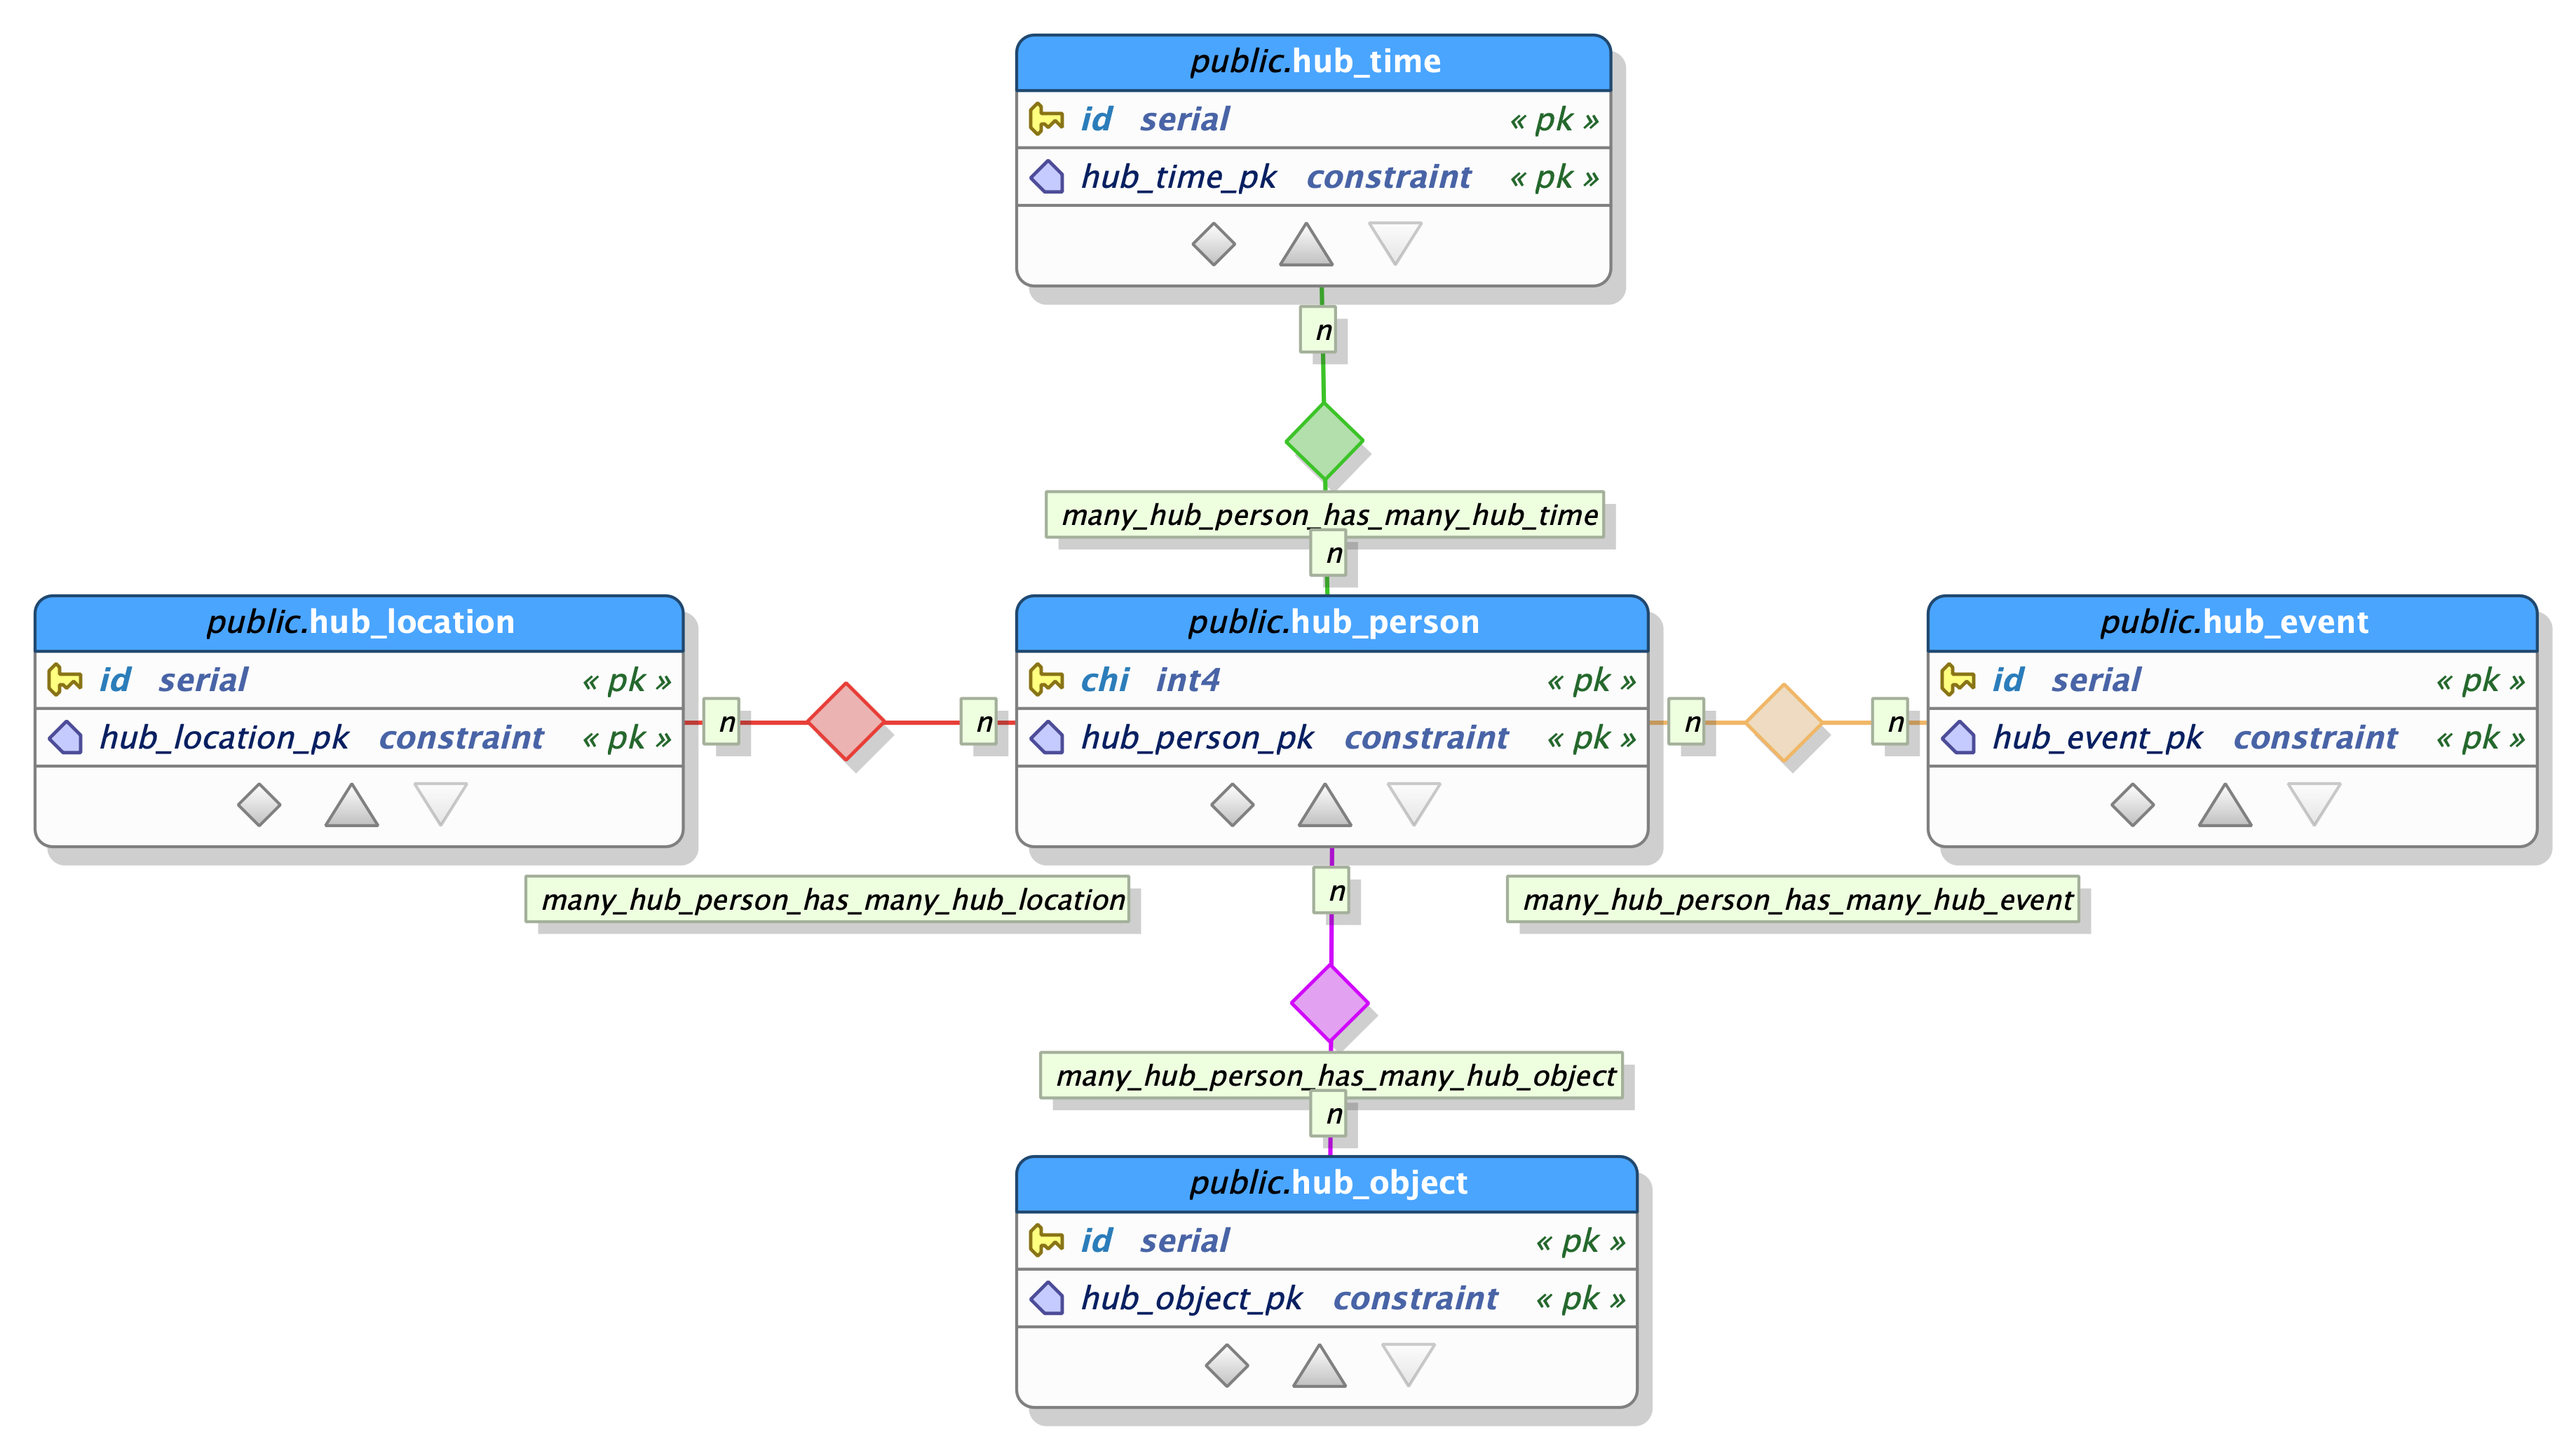
\includegraphics[width=10cm]{figures/technical/tpole_hubs.png}
    \caption{Data Vault - T-P-O-L-E Hubs}
    \label{fig:dvhubs}
\end{figure}

\item \emph{links} that represent associations or transactions between business keys (Hubs);

\begin{figure}[H]
    \centering
    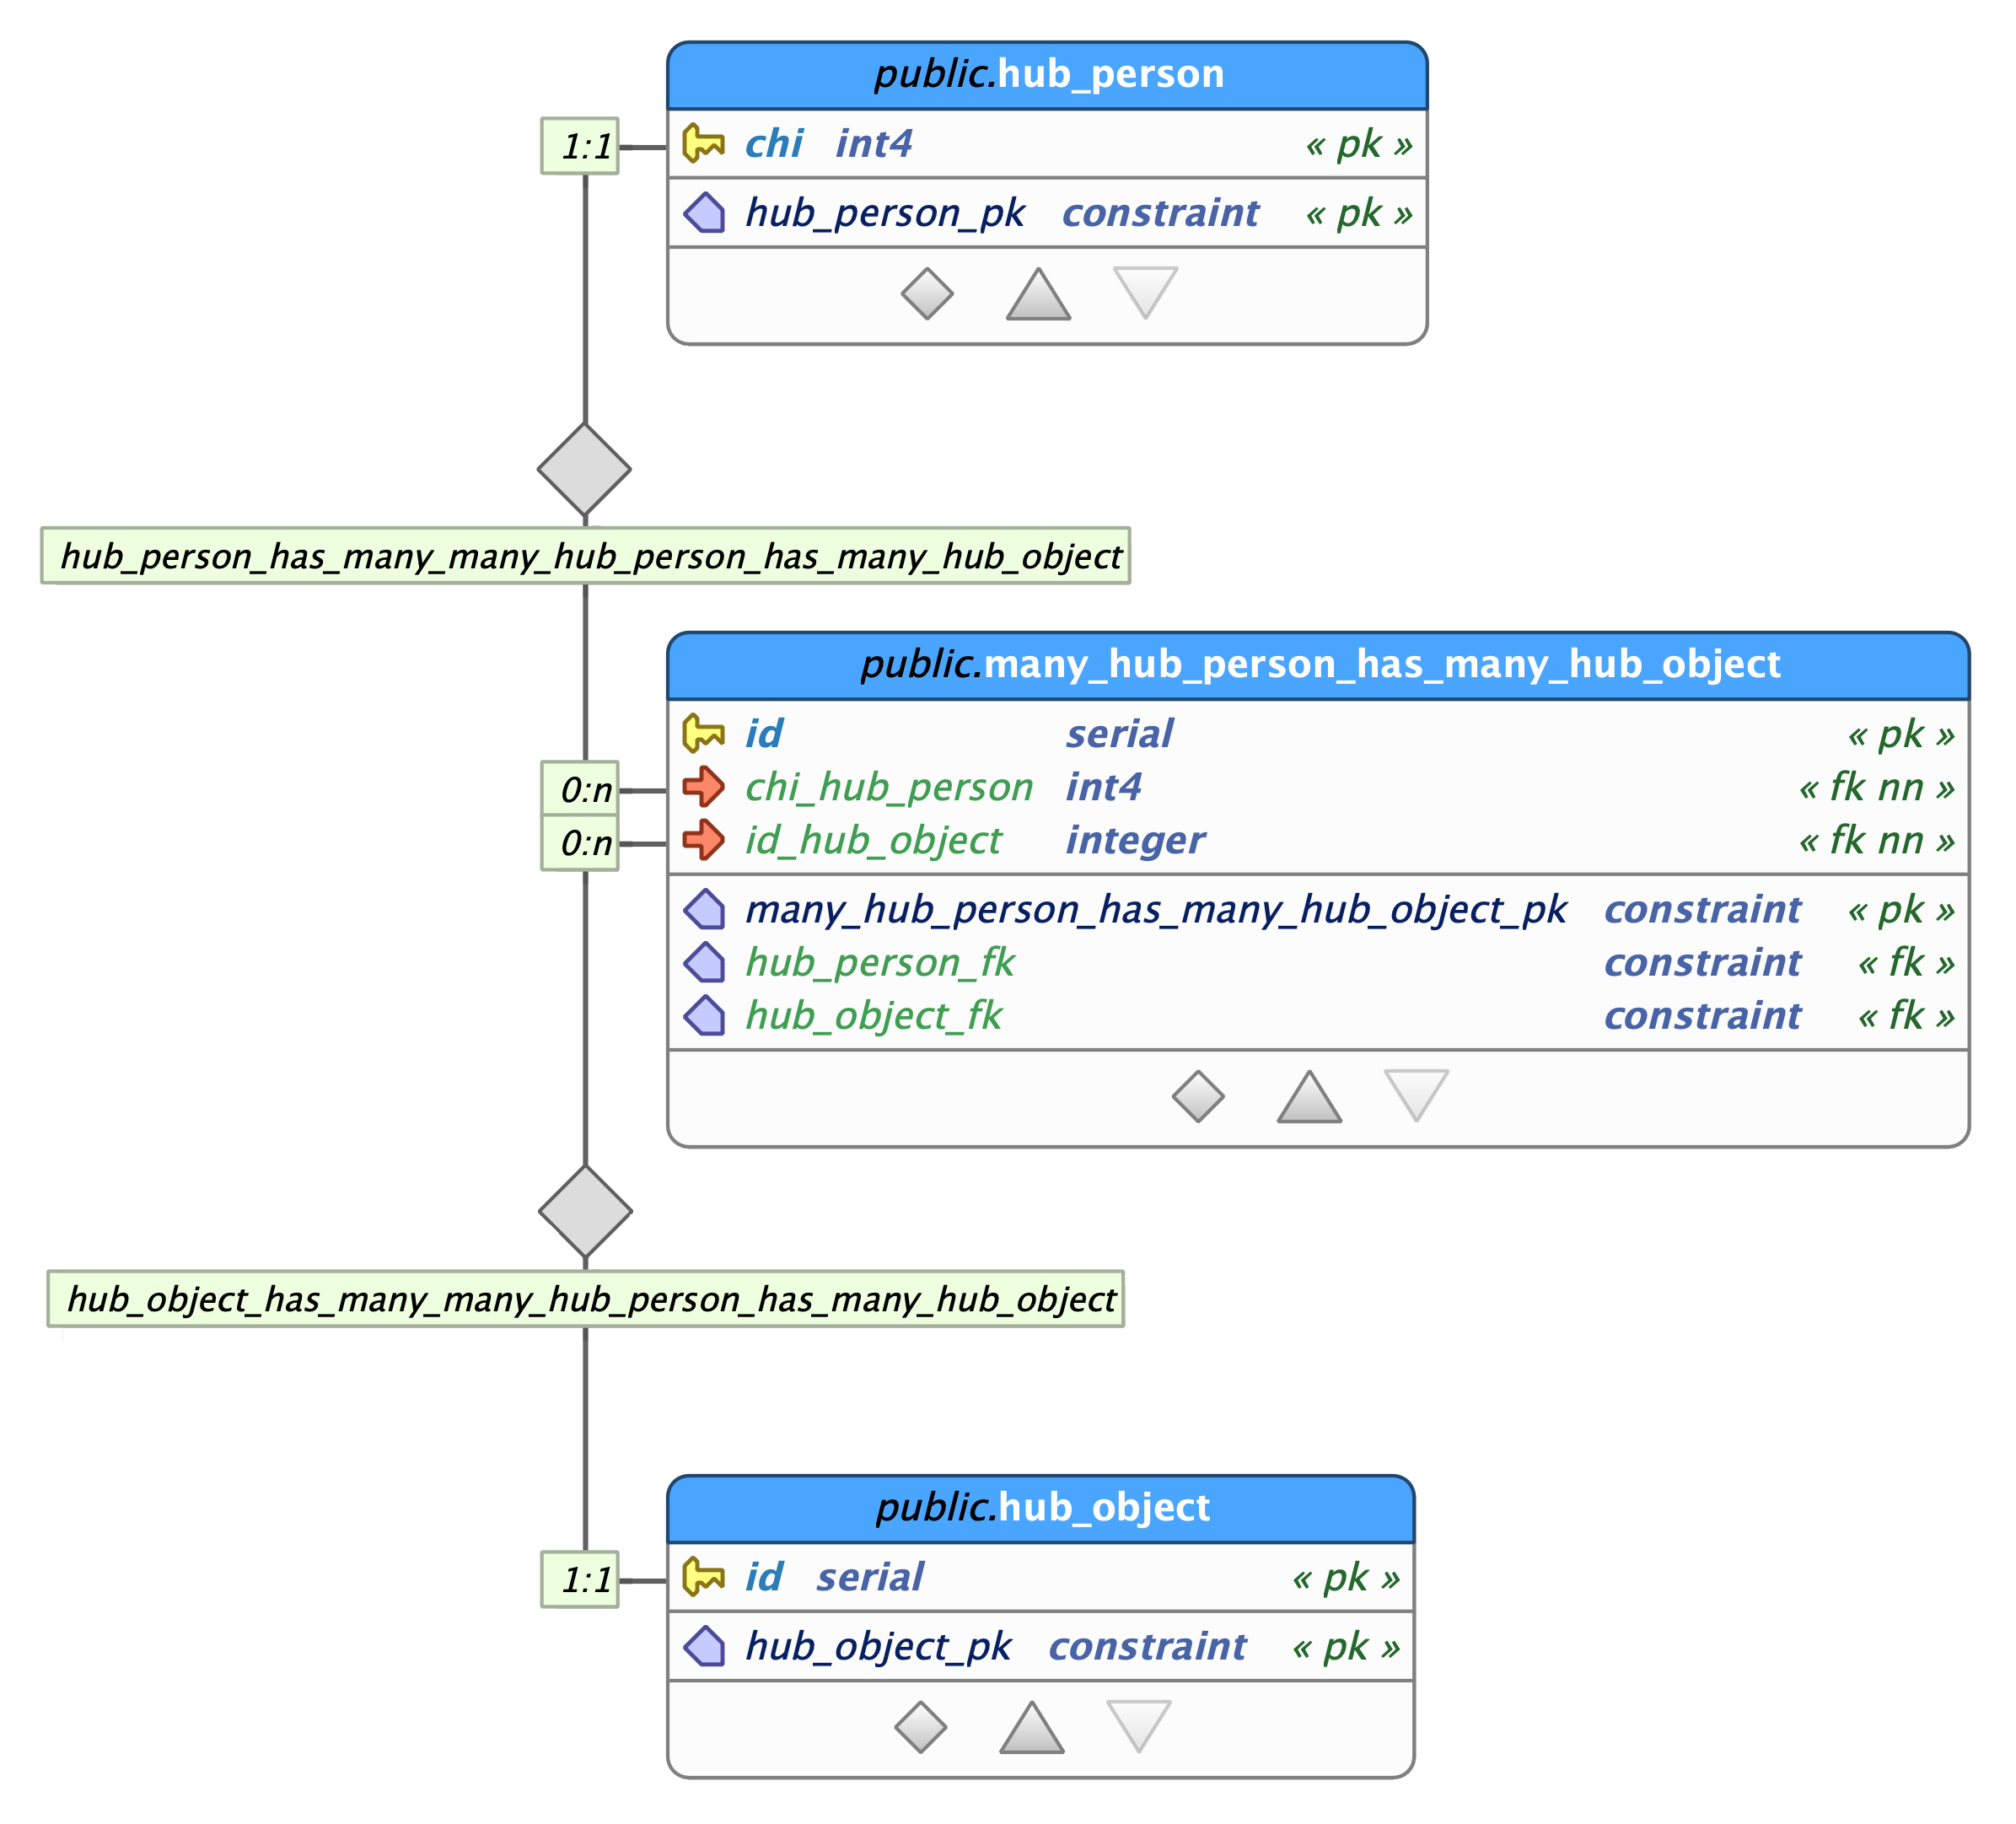
\includegraphics[width=10cm]{figures/technical/links.png}
    \caption{Data Vault - T-P-O-L-E Links}
    \label{fig:dvlinks}
\end{figure}

\item \emph{satellites}, where temporal and descriptive attributes of the hubs and links are stored;

%The hubs and links form the structure of the model, but holds neither temporal attributes nor descriptive attributes. These attributes are stored in separate tables called satellites.

\begin{figure}[H]
    \centering
    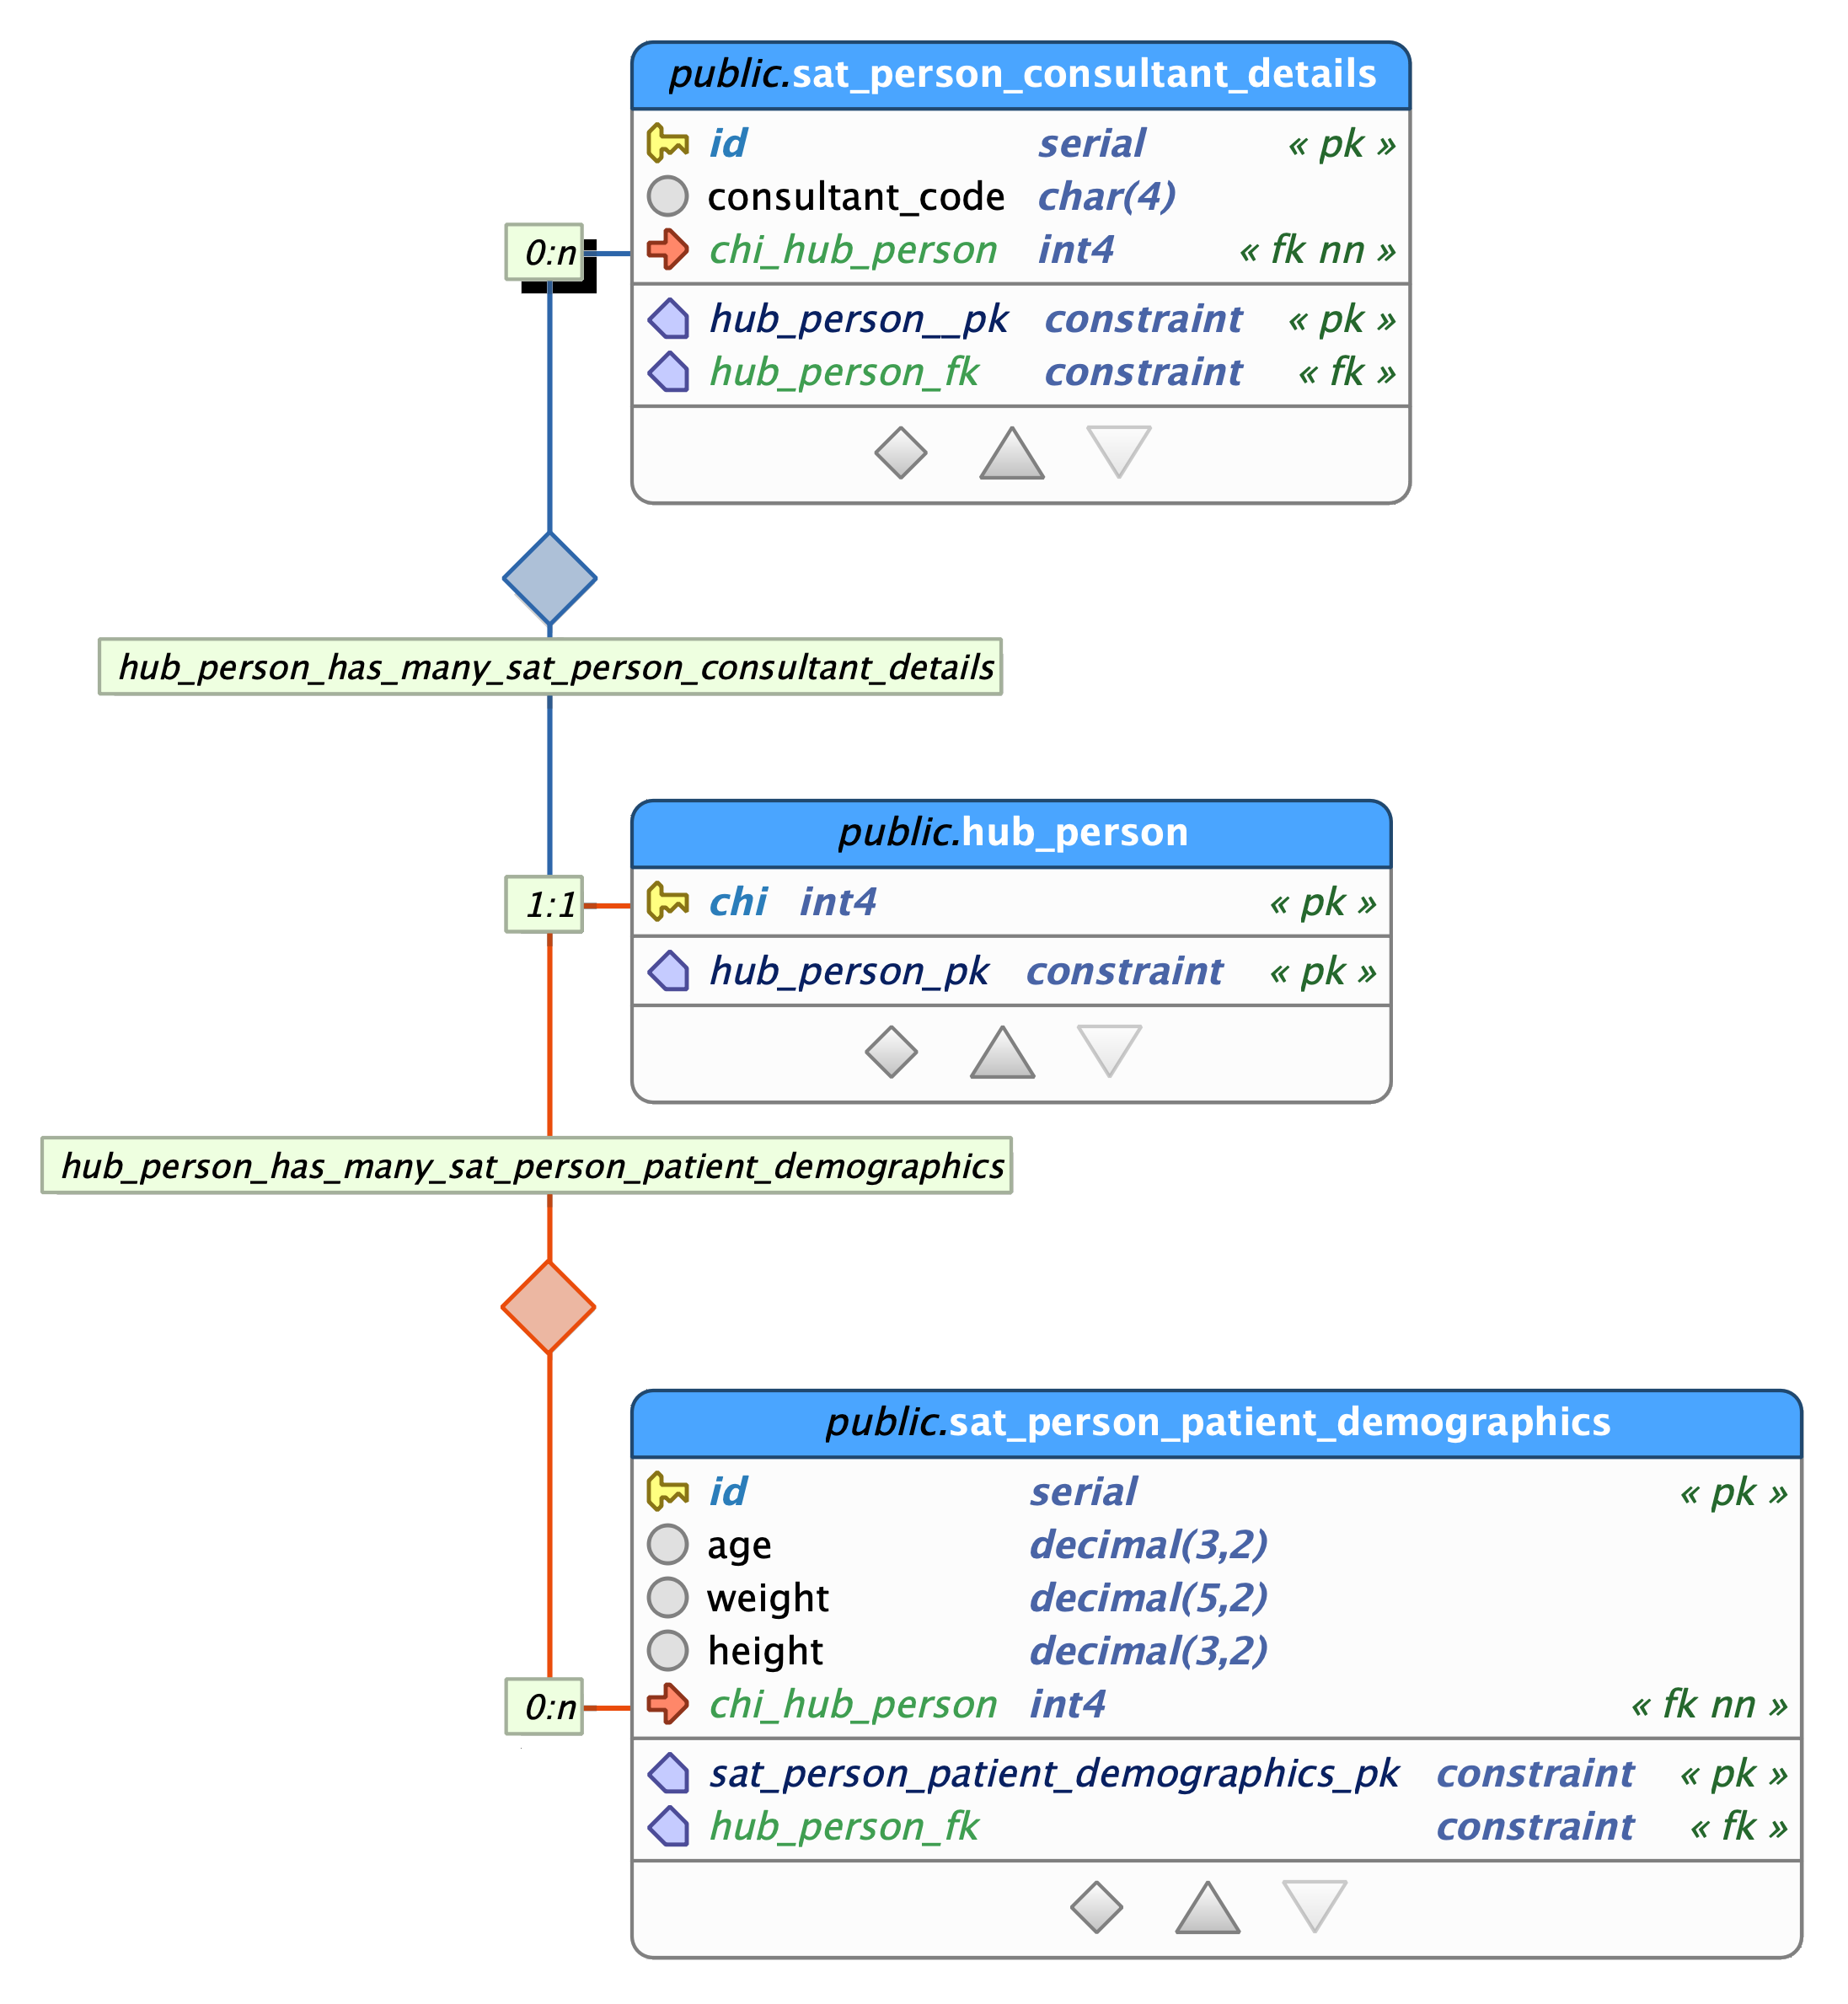
\includegraphics[width=10cm]{figures/technical/satellites.png}
    \caption{Data Vault - T-P-O-L-E Satellites}
    \label{fig:dvsatellites}
\end{figure}
\end{itemize}



\section{Reference tables}

Reference tables are a normal part of a healthy data vault model. These will hold look-ups and standards for common codes within the complete data vault.

This is the area where the standards are stored ready for the data vault to use during the upload.

\section{What is a T-P-O-L-E Data Vault?}

The Time-Person-Object-Location-Event (T-P-O-L-E) Data Vault is a highly specific data vault that reduces all business activities to be generalised as one of five types of hubs.

The hubs are:
\begin{itemize}
    \item Time Hub
    The time is sub-divided as Date and Time.
    Prescribes ISO 8601-1:2019 and ISO 8601-2:2019 as standards.
    
    \item Person Hub
    The person involve is record using concept of "Golden Nominal"
    This type of record is a single person record with a unique reference proven to that single person.
    
    \item Object Hub
    The objects are any other referable entities involved in the interaction.
    Examples are:
    \begin{itemize}
        \item Organisations (Legal entity of Bank, Hospital or School)
        \item Physical objects (Bank Card, Vehicle or hospital bed)
        \item Buildings (Physical Bank, Hospital or School)
    \end{itemize}
    \item Location Hub
    The location is to one thousandth of a latitude and longitude (i.e. to less than one square meter) using ISO 6709:2008 Standard. (\url{https://www.iso.org/standard/39242.html})
    
    Note that the location stores different descriptions via location satellites for the same location.
    
    Example: a location could be a building's location, physical address and a bus stop on a bus route at the same time.
    
    \item Event Hub
    The event is the individual action or event recorded.
    
\end{itemize}

The links are force to be only between these T-P-O-L-E hubs to limit the complexity of the core structure of the model. These links are different for each implementation of the T-P-O-L-E methodology but is high descriptive via meta-data how and what is stored in the links.

The satellites are connected to T-P-O-L-E hubs to add the temporal attributes and descriptive attributes.
These satellites holds all the attributes for a specific type of hub.
These common attributes between satellites are the concept that the specific values was valid from a specific point in time until another point in time.

Note: Data is never delete or modified as it is immutable. All transactions are inserts to indicate the latest state of the data. This creates a complete history with provenance and full lineage.

